\chapter{Plane Mirror Image Characteristics}

\section{Aim}
To investigate the properties of the image formed by a plane mirror

\section{Background Information}
Mirrors have a variety of uses and are often found in homes, saloons, cars and a variety of industrial applications. It is very interesting when you look at yourself in a mirror and see your own image. Images formed by plane mirrors have different properties. What are the relationships between the object and its image in a plane mirror?

\section{Materials}
Plane mirror, 3 optical pins, 4 drawing pins, plain paper, drawing board and ruler

\section{Procedure}
\begin{enumerate}
\item Fix a piece of plain paper onto a drawing board using drawing pins.
\item Draw a horizontal line LM at the center of the plain paper.
\item Place the plane mirror upright along the line LM.
\item Fix a pin at point O, 4 cm from the center N of the plane mirror as seen in Figure \ref{fig:plane-mirror-1}.
\item Fix two pins at points P and Q so as to appear in line with the image of O in the mirror. 
\item Mark the points and then remove the pins at P and Q.
\item Fix the two pins at points R and S on opposite side of ON to appear in line with the image of O in the mirror.
\item Mark the points on the paper and then remove the pins at points R and S. 
\item Draw a line through P and Q that extends across the line LM. Do the same for R and S. Label the intersection of these two lines as O’.
\item Join O and O’ with a line which cuts the reflecting surface at point N, measure and record the length of NO and NO’ as $u$ and $v$  respectively.
\item Change the position of object O by increasing it by intervals of 2 cm to obtain five more readings of $u$ and $v$. 
\end{enumerate}

\begin{figure}[h!]
\centering
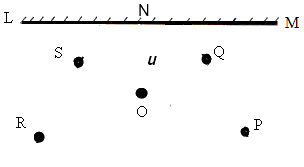
\includegraphics[width=8cm]{./img/plane-mirror-1.png}
\caption{Plane Mirror Image Characteristics practical setup}
\label{fig:plane-mirror-1}
\end{figure}

\section{Analysis and Interpretation}
\begin{enumerate}
\item What is the position of the image formed with respect to the mirror?
\item Plot the graph of $v$ against $u$. 
\item Determine the slope of the graph.
\item What is the physical meaning of the slope?
\item From the value of slope obtained comment on the size of the image formed by a plane mirror.
\end{enumerate}

\section{Conclusion}
From the experiment, explain about the characteristics of the image formed by a plane mirror.

\section{Questions for Discussion}
\begin{enumerate}
\item What would you see if you looked at the word \emph{\textbf{BABA}} in the plane mirror? What is this property called? 
\item If you see your friends in a mirror, can they see you at the same time?
\end{enumerate}

\section{Reflection and Self Assessment}
\begin{enumerate}
\item Apart from the uses mentioned in the introduction, where can the results of this experiment be used?
\item How can you use plane mirrors to see the back of your head?
\item What did you find most and least interesting about this experiment? Explain.
\end{enumerate}